% For PDF
%\documentclass[a4paper,onecolumn]{report}
% For double-sided printing
\documentclass[a4paper,openright,twoside,onecolumn]{report}

% Packages
\usepackage{multirow}
\usepackage{setspace}
\usepackage{afterpage}
\usepackage{amsmath}
\usepackage{amsfonts}
\usepackage{amssymb}
\usepackage{graphicx}
\usepackage[table,xcdraw]{xcolor}
\usepackage[utf8]{inputenc}
\usepackage{fancyhdr}
\usepackage{hyperref}
\usepackage{tocloft}
\usepackage{natbib}
\usepackage{changepage}
\usepackage{blindtext}
\usepackage{lipsum}
\usepackage[final]{pdfpages}
\usepackage{verbatim}
\usepackage{listings}
\usepackage{caption}
\usepackage{booktabs}
\usepackage[left=2cm,right=2cm,top=2cm]{geometry}

\hypersetup{
	colorlinks,
	linktoc=page,
	citecolor=red,
	filecolor=blue,
	linkcolor=blue,
	urlcolor=blue
}

\newcommand\blankpage{%
	\null
	\thispagestyle{empty}%
	\addtocounter{page}{-1}%
	\newpage}

% --- Document metadata ---
% Title page is going to render details from here
\title{My very important thesis topic}
\author{Anton Ashmarin}
\date{\today}

% --- Custom styles ---
\setcounter{tocdepth}{3}
\setcounter{secnumdepth}{3}

\makeatletter
\edef\mytitle{\@title}
\makeatother

\makeatletter
\edef\myself{\@author}
\makeatother

% Here we redefine page numeration
\renewcommand\thesection{\arabic{section}}
\renewcommand\thesubsection{\thesection.\arabic{subsection}}

\pagestyle{fancy}
\fancyhf{}
\fancyhead[LE,RO]{\mytitle}
\fancyhead[RE,LO]{CQF Institute}
\fancyfoot[CE,CO]{\nouppercase{\rightmark}}
\fancyfoot[LE,RO]{\thepage}

% --- Document begin ---
\begin{document}

% This way ToC and Bibliography appears like a Section, not Chapter, + center-aligned
\makeatletter
\renewcommand\tableofcontents{
  \section*{
    \center\contentsname
    \@mkboth{\MakeUppercase\contentsname}{\MakeUppercase\contentsname}}
  \@starttoc{toc}}
\makeatother

\makeatletter
\renewcommand\listoffigures{
  \section*{
    \center\listfigurename
    \@mkboth{\MakeUppercase\listfigurename}{\MakeUppercase\listfigurename}}
  \@starttoc{lof}}
\makeatother

\makeatletter
\renewcommand\listoftables{
  \section*{
    \center\listtablename
    \@mkboth{\MakeUppercase\listtablename}{\MakeUppercase\listtablename}}
  \@starttoc{lot}}
\makeatother

\makeatletter
\renewcommand\bibsection{
  \section*{
    \center\bibname
    \@mkboth{\MakeUppercase\refname}{\MakeUppercase\refname}}}
\makeatother

% --- Title page ---
\begin{titlepage}
    \newgeometry{top=1in,bottom=1in,right=0.5in,left=0.5in}
    
    \begin{center}

        \begin{figure}[!htb]
            \centering
            
\includegraphics[width=0.3\textwidth]{img/cqf_logo.png}
        \end{figure}
     
        \huge \textbf{Final Project}\\
        \vspace{0.5cm}
        \Large \textbf{\mytitle}\\
        \vspace{0.7cm}
        \large \textbf{\myself}\\
        \vspace{0.2cm}
        \textbf{January 2022 cohort}\\ 

        \mbox{}
        \vfill

        \begin{figure}[!htb]
            \centering
            
\includegraphics[width=0.2\textwidth]{img/FitchLearning_logo.png}
        \end{figure}

        \today
    \end{center}

% Blank page left for printing
\afterpage{\blankpage}
\end{titlepage} 

% --- Abstract ---
% Default tex abstract rendering is not the best, so we redefine it

\fancypagestyle{plain}{}
\begin{center}
    \Large \textbf{Abstract}
\end{center}

\begin{adjustwidth}{50pt}{50pt}

Brief summary of the project goes here.

\end{adjustwidth}

\pagenumbering{arabic}
\setcounter{page}{2}

% --- Table of contents ---
{\let\clearpage\relax} % To remove pagebreak
\fancypagestyle{plain}{}
\begin{spacing}{1.2}
	\tableofcontents
	\listoffigures
	\listoftables
\end{spacing}

\newpage

% --- Document body ---
% Please put all the content here. Note \section{} is the highest level of header hierarchy.
%\include{content file you want to render from the new page}
%\input{content file you want to render without page breaks}

% This is a sample content just for reference

\section{Introduction}

This is how you reference pictures in the text: (Figure ~\ref{fig:figure1}) \\
This is how you cite: \cite[Some page, some paraghaph]{hawking1988} \\
This is how you create nice tables, and reference them (See table ~\ref{table:tab1})

\begin{table}[ht]
    \captionof{table}{Assets selected for portfolio}
    \label{table:tab1}
    \begin{tabular}{@{}rrrrrr@{}}
    \toprule
    \textbf{Ticker} & \textbf{Company name}      & \boldmath{$\beta$} & \textbf{Sector}        & \textbf{Industry}  \\ 
    \midrule
    WMT       & Walmart Inc.            & 0.507262      & Consumer Defensive     & Discount Stores                  \\
    XOM       & Exxon Mobil Corporation & 0.936712      & Energy                 & Oil \& Gas Integrated               \\
    TSLA      & Tesla, Inc.             & 1.43901       & Consumer Cyclical      & Auto Manufacturers                \\
    NEM       & Newmont Corporation     & 0.292796      & Basic Materials        & Gold                                \\
    KR        & Kroger Company (The)    & 0.311054      & Consumer Defensive     & Grocery Stores                      \\
    GIS       & General Mills, Inc.     & 0.379007      & Consumer Defensive     & Packaged Foods                       \\
    META      & Meta Platforms, Inc.    & 1.201507      & Communication Services & Internet Content \& Information     \\
    MRNA      & Moderna, Inc.           & 0.456853      & Healthcare             & Biotechnology                     \\ 
    \bottomrule
    \end{tabular}
\end{table}

\begin{figure}[ht]
    \begin{center}
        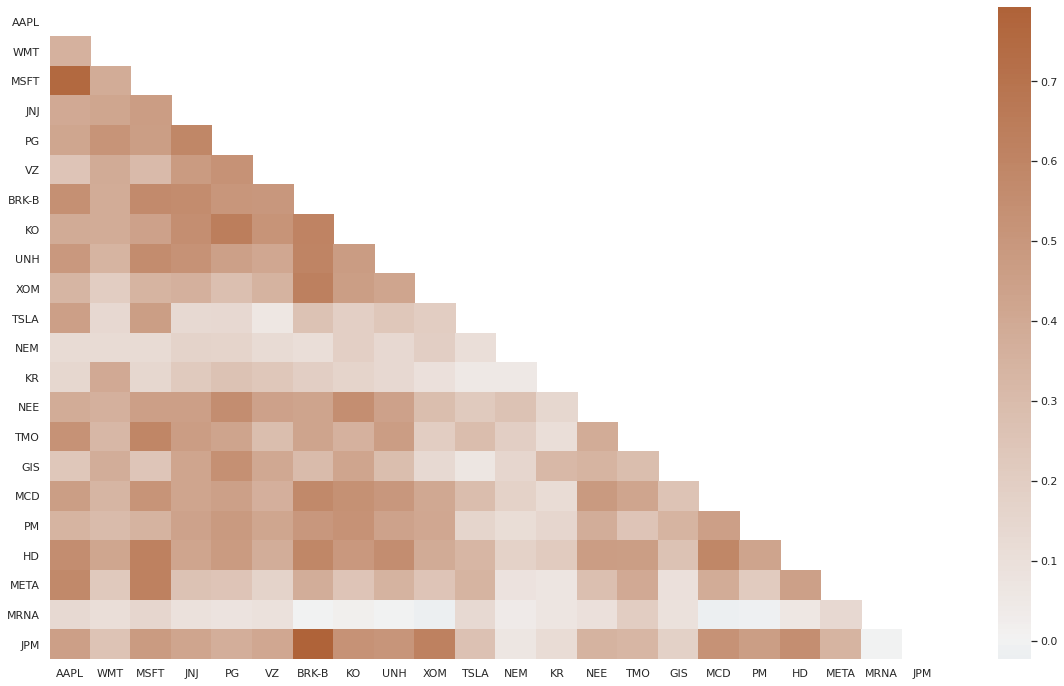
\includegraphics[width=0.8\textwidth]{img/fig1.png}
        \caption{Picture description}
        \label{fig:figure1}
    \end{center}
\end{figure}

This is how you do math and reference equations (\ref{eq:1}):

\begin{equation} \label{eq:1}
    w^*=\frac{\Sigma^{-1}(\mu_{BL}-r_f\mathbf{1})}{\mathbf{1}^T\Sigma^{-1}(\mu_{BL}-r_f\mathbf{1})}   
\end{equation}

$$
E = mC^2
$$

This is how you inline math: 
$\quad \dfrac{\partial L}{\partial \omega}(\omega, \lambda, \gamma) = \omega'\Sigma - \lambda\mu' - \gamma\mathbf{1}' = 0 \quad$ 
in the normal text

This is how you do bullet lists:

\begin{itemize}
    \item Item 1
    \item Item 2
    \item Item 3
\end{itemize}

Or numbered lists:

\begin{enumerate}
    \item Item
    \item Item
    \item Item
\end{enumerate}

\noindent
New paragraph with no indent. New paragraph with no indent. New paragraph with no indent. New paragraph with no indent. New paragraph with no indent. New paragraph with no indent. New paragraph with no indent.

Paragraph with indent. Paragraph with indent. Paragraph with indent. Paragraph with indent. Paragraph with indent. Paragraph with indent. Paragraph with indent. Paragraph with indent. Paragraph with indent. Paragraph with indent.


\newpage
\section{Methods}
\section{Research Body}
\subsection{Very Important Topic 1}
\subsubsection{Item 1}
\subsubsection{Item 2}
\subsubsection{Item 3}
\newpage
\subsection{Very Important Topic 2}
\newpage
\section{Conclusion}

% --- Bibliography ---

\newpage
\addcontentsline{toc}{section}{\protect\numberline{}\bibname}
\bibliographystyle{plain}
\fancypagestyle{plain}{}
\renewcommand{\bibname}{References}
\nocite{*} % list all refs in database, cited or not
\bibliography{ref}

% --- Appendix ---

\appendix

\addcontentsline{toc}{section}{Appendicies}

\phantomsection\label{Setup}
\addcontentsline{toc}{subsection}{Environment setup}
\section*{Environment setup}

To run the Jupyter notebook install dependencies:

\begin{lstlisting}[language=bash]
pip install -r requirements.txt
\end{lstlisting}

% Include plain text in the report
\verbatiminput{res/requirements.txt}


\newpage
\phantomsection\label{SomePdf}
\addcontentsline{toc}{subsection}{Supplied pdf document}
% Note: pdf will be rendered as is, without the page numbers and styles

\includepdf[pages=-]{res/some.pdf}

% --- Document end ---
\end{document}